% Cartoon of how the vortices lose energy (TikZ; \input from notes.tex inside a figure environment).
% Colours as in the data figures: grey = zonal flow, orange = exchange with the jets, green = conversion to entropy,
% red = the velocity-space sink.
\definecolor{cjet}{gray}{0.45}
\definecolor{csup}{HTML}{FF7F0E}
\definecolor{cent}{HTML}{2CA02C}
\definecolor{crem}{HTML}{D62728}
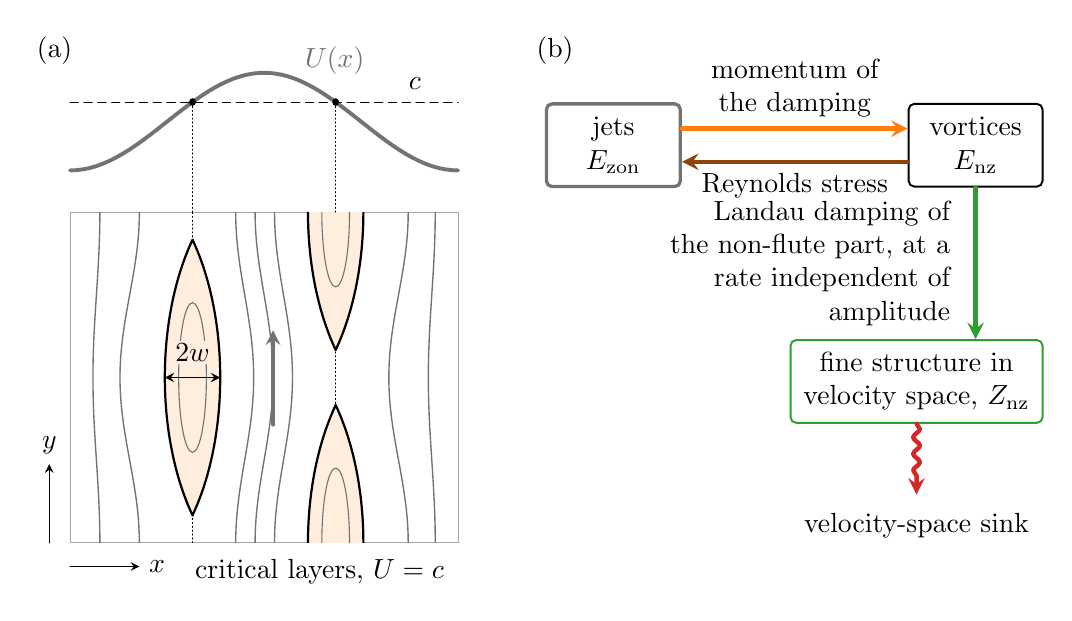
\begin{tikzpicture}[x=1cm, y=1cm, >=stealth, line cap=round, line join=round]
% ---------------------------------------------------------------- (a) geometry
\begin{scope}[xscale=0.88]
  \node[anchor=north west] at (-0.62, 6.55) {(a)};
  % zonal flow profile and phase speed
  \draw[cjet, line width=1.4pt] plot[domain=0:5.6, samples=60] (\x, {5.35 + 0.62*cos(deg(2*pi*(\x-2.8)/5.6))});
  \draw[densely dashed] (0, 5.598) -- (5.6, 5.598);
  \node[anchor=west, cjet] at (3.25, 6.12) {$U(x)$};
  \node[anchor=west] at (4.75, 5.83) {$c$};
  \fill (1.767, 5.598) circle (1.4pt); \fill (3.833, 5.598) circle (1.4pt);
  % the (x, y) plane
  \draw[black!35] (0, 0) rectangle (5.6, 4.2);
  \begin{scope}
    \clip (0, 0) rectangle (5.6, 4.2);
    % critical layers
    \draw[densely dotted] (1.767, 0) -- (1.767, 4.2); \draw[densely dotted] (3.833, 0) -- (3.833, 4.2);
    % cat's eyes: one per wavelength on each flank, staggered by half a wavelength (the shear changes sign)
    \foreach \yc in {2.1}
      \filldraw[fill=csup!14, draw=black, line width=0.8pt] (1.767, \yc-1.75) .. controls (2.30, \yc-0.75) and (2.30, \yc+0.75) .. (1.767, \yc+1.75)
        .. controls (1.234, \yc+0.75) and (1.234, \yc-0.75) .. cycle;
    \foreach \yc in {0, 4.2}
      \filldraw[fill=csup!14, draw=black, line width=0.8pt] (3.833, \yc-1.75) .. controls (4.366, \yc-0.75) and (4.366, \yc+0.75) .. (3.833, \yc+1.75)
        .. controls (3.300, \yc+0.75) and (3.300, \yc-0.75) .. cycle;
    % trapped orbits
    \draw[black!55, line width=0.4pt] (1.767, 2.1) ellipse (0.20 and 0.95);
    \draw[black!55, line width=0.4pt] (3.833, 0) ellipse (0.20 and 0.95); \draw[black!55, line width=0.4pt] (3.833, 4.2) ellipse (0.20 and 0.95);
    % open streamlines: the jet core and the two outer regions
    \foreach \xo/\am in {2.52/-0.13, 2.80/-0.13, 3.08/-0.13}
      \draw[cjet, line width=0.5pt] plot[domain=0:4.2, samples=40] ({\xo + \am*cos(deg(2*pi*\x/4.2))}, \x);
    \foreach \xo/\am in {0.38/0.05, 0.86/0.14}
      \draw[cjet, line width=0.5pt] plot[domain=0:4.2, samples=40] ({\xo + \am*cos(deg(2*pi*\x/4.2))}, \x);
    \foreach \xo/\am in {4.74/0.14, 5.22/0.05}
      \draw[cjet, line width=0.5pt] plot[domain=0:4.2, samples=40] ({\xo + \am*cos(deg(2*pi*\x/4.2))}, \x);
  \end{scope}
  % links between the profile and the plane
  \draw[densely dotted] (1.767, 4.2) -- (1.767, 5.598); \draw[densely dotted] (3.833, 4.2) -- (3.833, 5.598);
  % labels
  \draw[->, cjet, line width=1.3pt] (2.93, 1.50) -- (2.93, 2.70);
  \draw[<->, line width=0.5pt] (1.367, 2.1) -- (2.167, 2.1);
  \node[fill=csup!14, inner sep=1pt] at (1.767, 2.42) {$2w$};
  \draw[->] (0, -0.3) -- (1.0, -0.3) node[anchor=west] {$x$};
  \draw[->] (-0.3, 0) -- (-0.3, 1.0) node[anchor=south] {$y$};
  \node[anchor=north] at (3.6, -0.08) {critical layers, $U = c$};
\end{scope}
% ---------------------------------------------------------------- (b) energy flow
\begin{scope}[xshift=5.95cm,
    box/.style={draw, rounded corners=2pt, line width=0.7pt, align=center, inner sep=4pt, minimum height=1.05cm}]
  \node[anchor=north west] at (-0.15, 6.55) {(b)};
  \node[box, draw=cjet, line width=1.2pt, minimum width=1.7cm] (J) at (0.95, 5.05) {jets\\$E_\mathrm{zon}$};
  \node[box, minimum width=1.7cm] (V) at (5.55, 5.05) {vortices\\$E_\mathrm{nz}$};
  \node[box, draw=cent, minimum width=3.2cm] (F) at (4.80, 2.05) {fine structure in\\velocity space, $Z_\mathrm{nz}$};
  % exchange with the jets
  \draw[->, csup, line width=1.6pt] ([yshift=6pt]J.east) -- node[above, text=black, align=center] {momentum of\\the damping} ([yshift=6pt]V.west);
  \draw[<-, csup!55!black, line width=1.6pt] ([yshift=-6pt]J.east) -- node[below, text=black] {Reynolds stress} ([yshift=-6pt]V.west);
  % kinetic removal
  \draw[->, cent, line width=1.6pt] (V.south) -- (V.south |- F.north);
  \node[anchor=east, align=right] at (5.35, 3.55) {Landau damping of\\the non-flute part, at a\\rate independent of\\amplitude};
  \draw[->, crem, line width=1.6pt, decorate, decoration={snake, amplitude=1.2pt, segment length=6pt, post length=4pt}] (F.south) -- ++(0, -0.9);
  \node[anchor=north] at (4.80, 0.50) {velocity-space sink};
\end{scope}
\end{tikzpicture}
